
\section{Overview}
\label{sec:overview}

\begin{figure}[h]
  \centering
  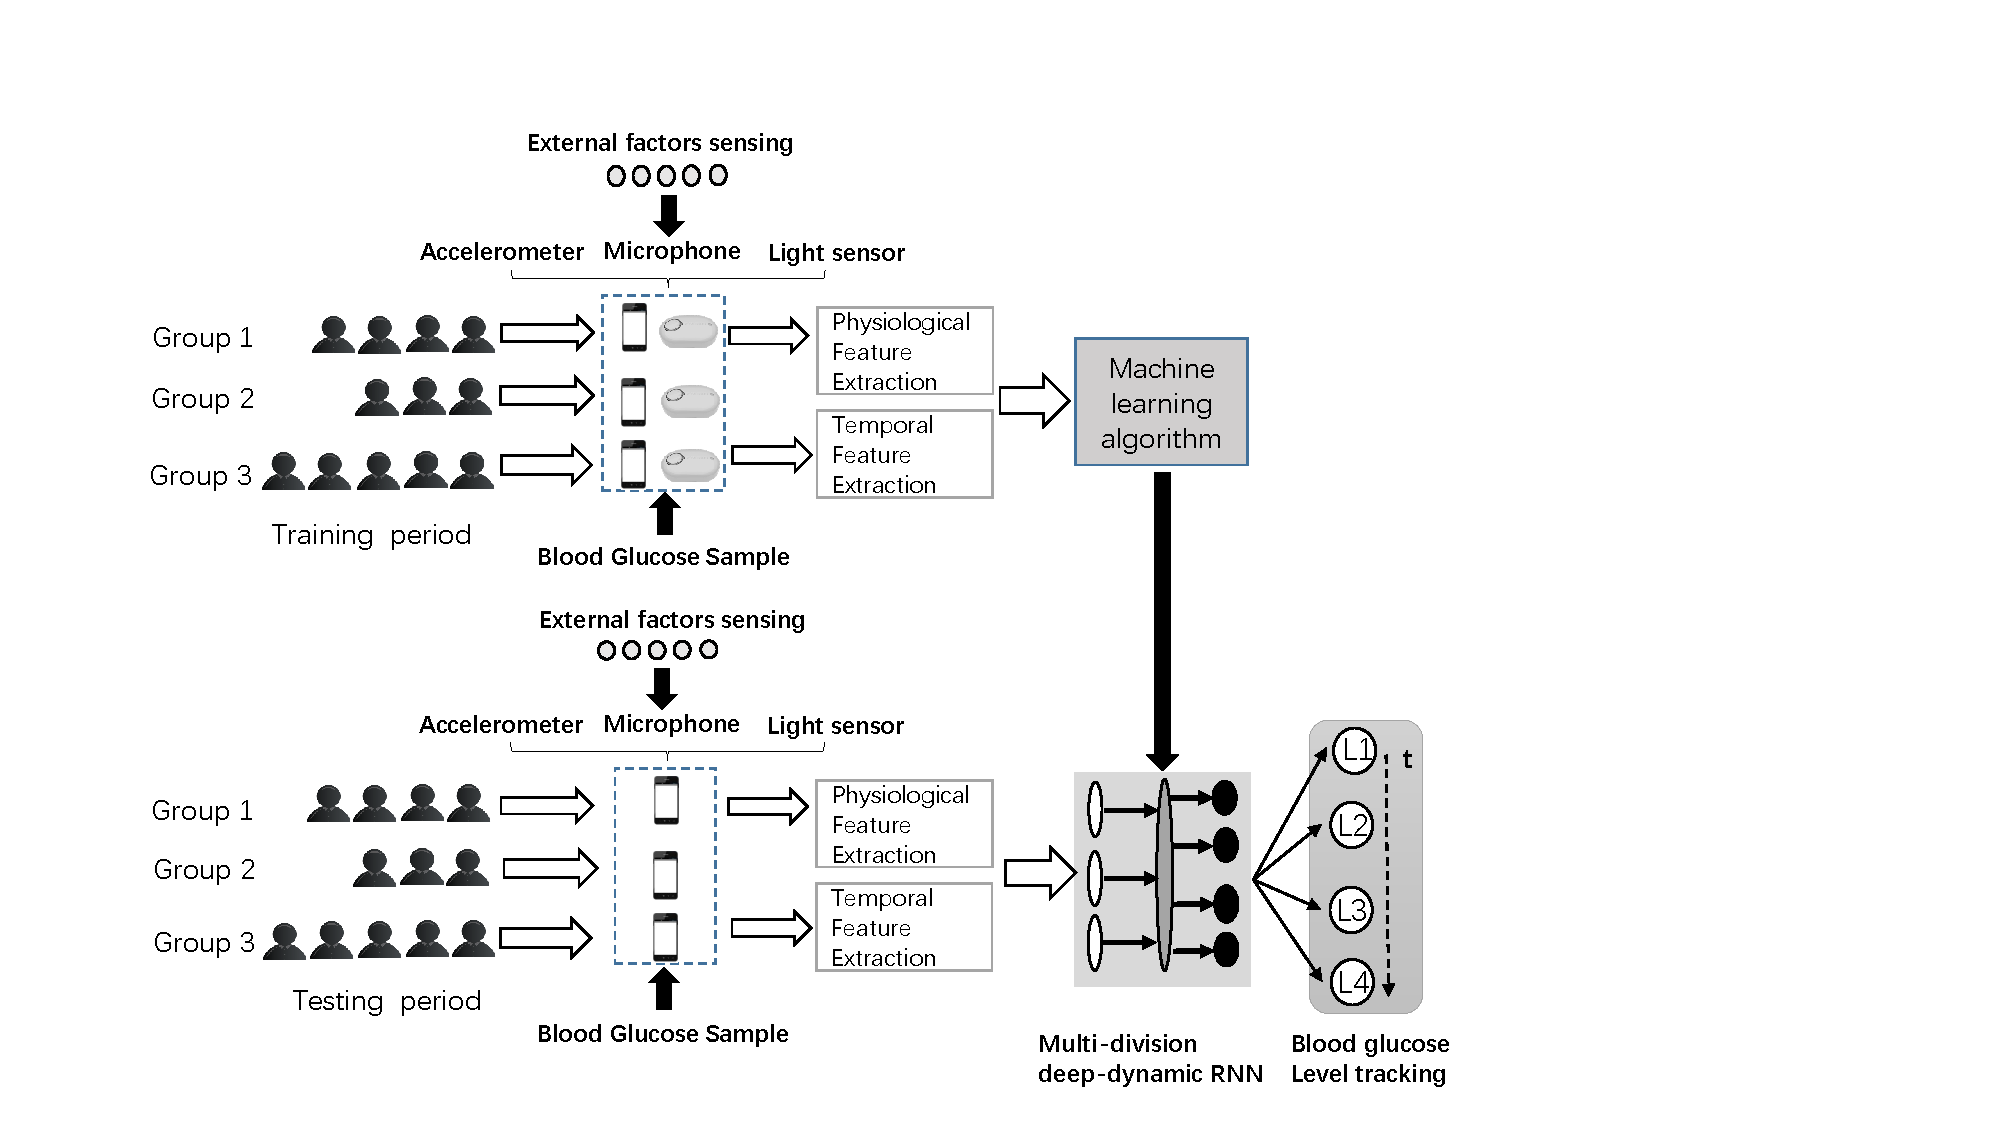
\includegraphics[width=0.85\columnwidth]{./img/System_Arch1.pdf}
  \caption{Architecture of \sysname. \TODO{may need redraw}}
  \label{fig:architecture}
\end{figure}

\sysname is a smartphone-based blood glucose level tracking system that \emph{(i)} collects important external impacting factors, \emph{(ii)} efficiently trains a personalized blood glucose level model via a multi-task deep learning framework (\modelname), and \emph{(iii)} timely reminds users of abnormal blood glucose levels.
\figref{fig:architecture} shows the architecture of \sysname, which consists of three modules.

The \textbf{external factor collection} module records important factors that are important to infer blood glucose concentration and convenient to input via smartphones.
The user is required to manually input their basic information (\eg health status, age, weight), and record drug, insulin and food intake.
Meanwhile, \sysname will automatically measure the physical activities and sleep quality of the user via embedded sensors.
After collecting data from multiple users, the \textbf{multi-task deep learning} framework (\modelname) first learns feature representations from users in the same group (non-diabetic, type I and type II diabetic), and then adopts a deep RNN layer to learn a general blood glucose level model on the dataset of all users.
Finally it outputs a personalized blood glucose level model for each individual via a personality layer.
The \textbf{blood glucose level tracking} module inputs measurements of the external factors into the trained personalized blood glucose level model, and outputs a specific blood glucose level at each time stamp.
In \sysname, we consider 4 blood glucose levels as in \tabref{tab:blood_glucose_levels}.

\begin{table}[h]
  \centering
  \caption{Normal and abnormal blood glucose levels~\cite{bib:BGWiKi}. The normal blood glucose concentration ranges from 4.4 mmol/L to 6.1 mmol/L. The blood glucose can grow to 7.8 mmol/L after eating. Blood glucose above 7.8 mmol/L for a prolonged period indicates the risk of diabetes mellitus. Blood glucose below 4.4 mmol/L is a sign of hypoglycemia.}
  \label{tab:blood_glucose_levels}
  \begin{tabular}{|c|c|c|}
  \hline
  \textbf{Blood Glucose Value (mmol/L)} & \textbf{Glocose Level} & \textbf{Explanation}                      \\ \hline
  (0, 4.4{]}                            & Level 1                & Low blood glucose (hypoglycemia)         \\ \hline
  (4.4, 6.1{]}                          & Level 2                & Normal level of fasting blood glucose      \\ \hline
  (6.1, 7.8{]}                          & Level 3                & Normal level of postprandial blood glucose \\ \hline
  (7.8, $+\infty$)                      & Level 4                & High blood glucose (hyperglycemia)          \\ \hline
  \end{tabular}
\end{table}


%The framework of \sysname is shown as \figref{fig:architecture}, consisting of four major components.
%The first one is the external factors collection.
%The users are required to enter their basic information into application, including of the age, the gender, the diabetes type and the year of diagnosis.

%After a user measures his/her blood glucose by a CGM, the records of the blood glucose along with the outer contextual factors occurred during the measurement are uploaded to an individual database automatically.
%Afterwards, a RNN model is trained based on the dataset to establish the relationships between the outer contextual factors and the corresponding blood glucose level.
%It then is fed into the user's smartphone.
%When the user does not wear the CGM, \sysname detects the outer contextual factors with embedded sensors in the smartphones, and infers the current blood glucose level based on the trained model.
%Once \sysname detects the abnormal points of blood glucose ( \ie in a \emph{high} or \emph{low} blood glucose level ), it reminds the user to measure the blood glucose by a clinical CGM for a further control.

%The extraction mechanisms of outer contextual factors are detailed as follows.
%
%\emph{Physical activity}:
%\sysname leverages the accelerometer to detect the user's activities by the approaches in \cite{bayat2014study}, as well as the corresponding time costs.
%\sysname then measures the calorie of user's physical consumption.
%
%\emph{Food intake}:
%\sysname measures the food's effect on a person's blood glucose level based on the glycemic index.
%
%\emph{Clinical drug intake}:
%\sysname records the name and amount of the drug that user eat.
%
%\emph{Time}:
%\sysname invokes the timer embedded in the smartphone to record the time.
%
%\emph{Sleep quality}:
%\sysname measures the user's sleep by the approach in \cite{gu2014intelligent}.
